
% webcml functionality
\begin{frame}
  \frametitle{Introduction}
\begin{itemize_loose}
\item The purpose of this tutorial is to introduce the user to submitting jobs to the WCTC web interface.

\item A CML error-rate simulation of BPSK modulation in an AWGN channel is submitted as a WCTC job.

\item The job results are saved to the user's local machine and plotted using CML.
\end{itemize_loose}

\end{frame}


\begin{frame}
\frametitle{Assumptions}
In this tutorial, it is assumed that the user has
\begin{itemize_loose}
\item A working MATLAB version $\geq$ 7.6 (R2008a)
\item Downloaded the WCRL Coded Modulation Library (CML) from \url{http://code.google.com/p/iscml/wiki/cml}.
\item Installed CML into local directory $<$CMLROOT$>$.
\item Followed the quickstart tutorial on the download site to familiarize with fundamental CML concepts.
\item Created a WCTC Web Interface Account as described in Section 3.
\end{itemize_loose}

\end{frame}

% tutorial terminology
\begin{frame}
\frametitle{Terminology}
The following terminology will be used throughout the tutorial:
\begin{itemize_loose}
\item Local computer - The user's computer running CML.
\item $<$CMLROOT$>$ - Directory on user's local computer containing CML.
\item Cluster - The server infrastructure administered by WCRL which hosts WCTC.
\item Job File - File generated by CML which contains the parameters of a single simulation for submission to using the WCTC web interface.
\end{itemize_loose}
\end{frame}


% starting cml
\begin{frame}
  \frametitle{ Starting CML }

  \begin{itemize}
  \item Start MATLAB and cd to $<$CMLROOT$>$.
  \item Execute function CmlStartup() to initialize CML.
  \end{itemize}

  \begin{figure}
    \centering
    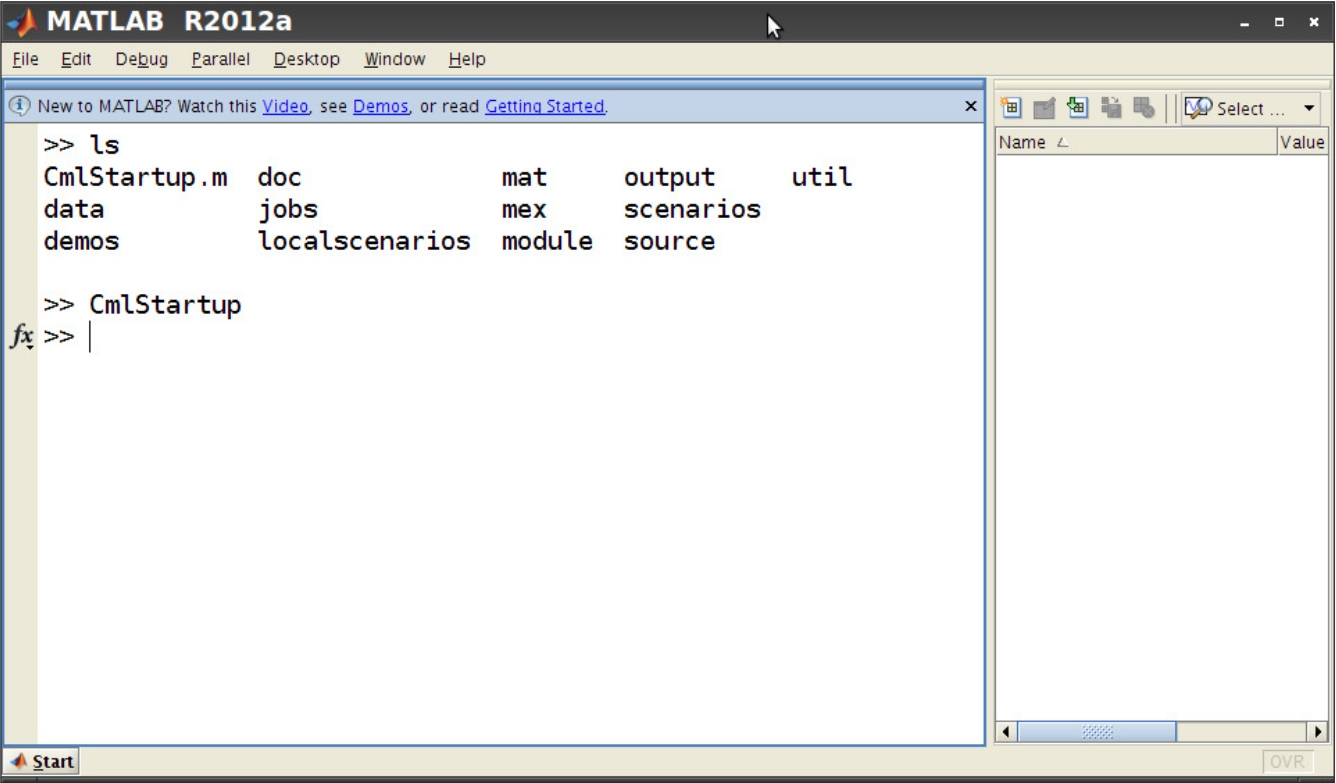
\includegraphics[width=.8\textwidth]{cml_startup}
  \end{figure}

\end{frame}




% creating a job file
\begin{frame}
  \frametitle{ Creating a Job File }

  In this example, we create a job file for an error-rate simulation of uncoded BPSK in AWGN.
  \begin{itemize}
  \item Scenario: UncodedScenarios
  \item Record: 1
  \end{itemize}

  \begin{figure}
    \centering
    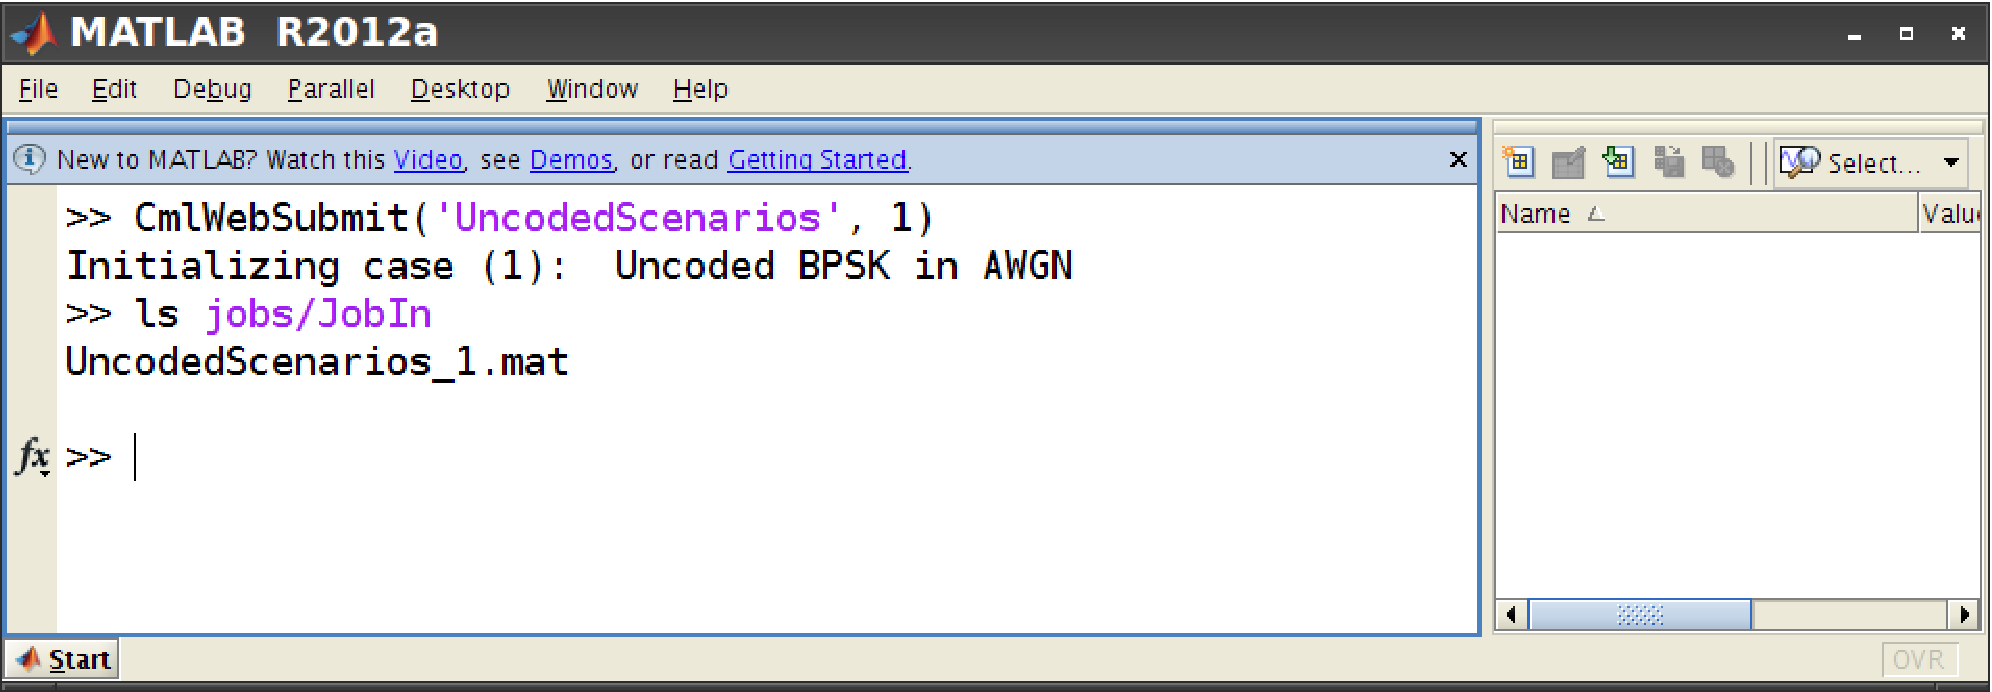
\includegraphics[width=.8\textwidth]{cml_websubmit}
  \end{figure}

  \begin{itemize}
  \item CmlWebSubmit() has created the job file $<$CMLROOT$>$/jobs/JobIn/UncodedScenarios\_1.mat
  \end{itemize}

\end{frame}




% web interface login
\begin{frame}
  \frametitle{WCTC Web Interface Login}

  \begin{itemize_loose}
  \item To submit the generated job file, log in to the WCTC web interface located at
    \\ \url{http://wctc.csee.wvu.edu}
  \item Use the credentials created in Section 2.
  \end{itemize_loose}

  \centering
  \begin{figure}
    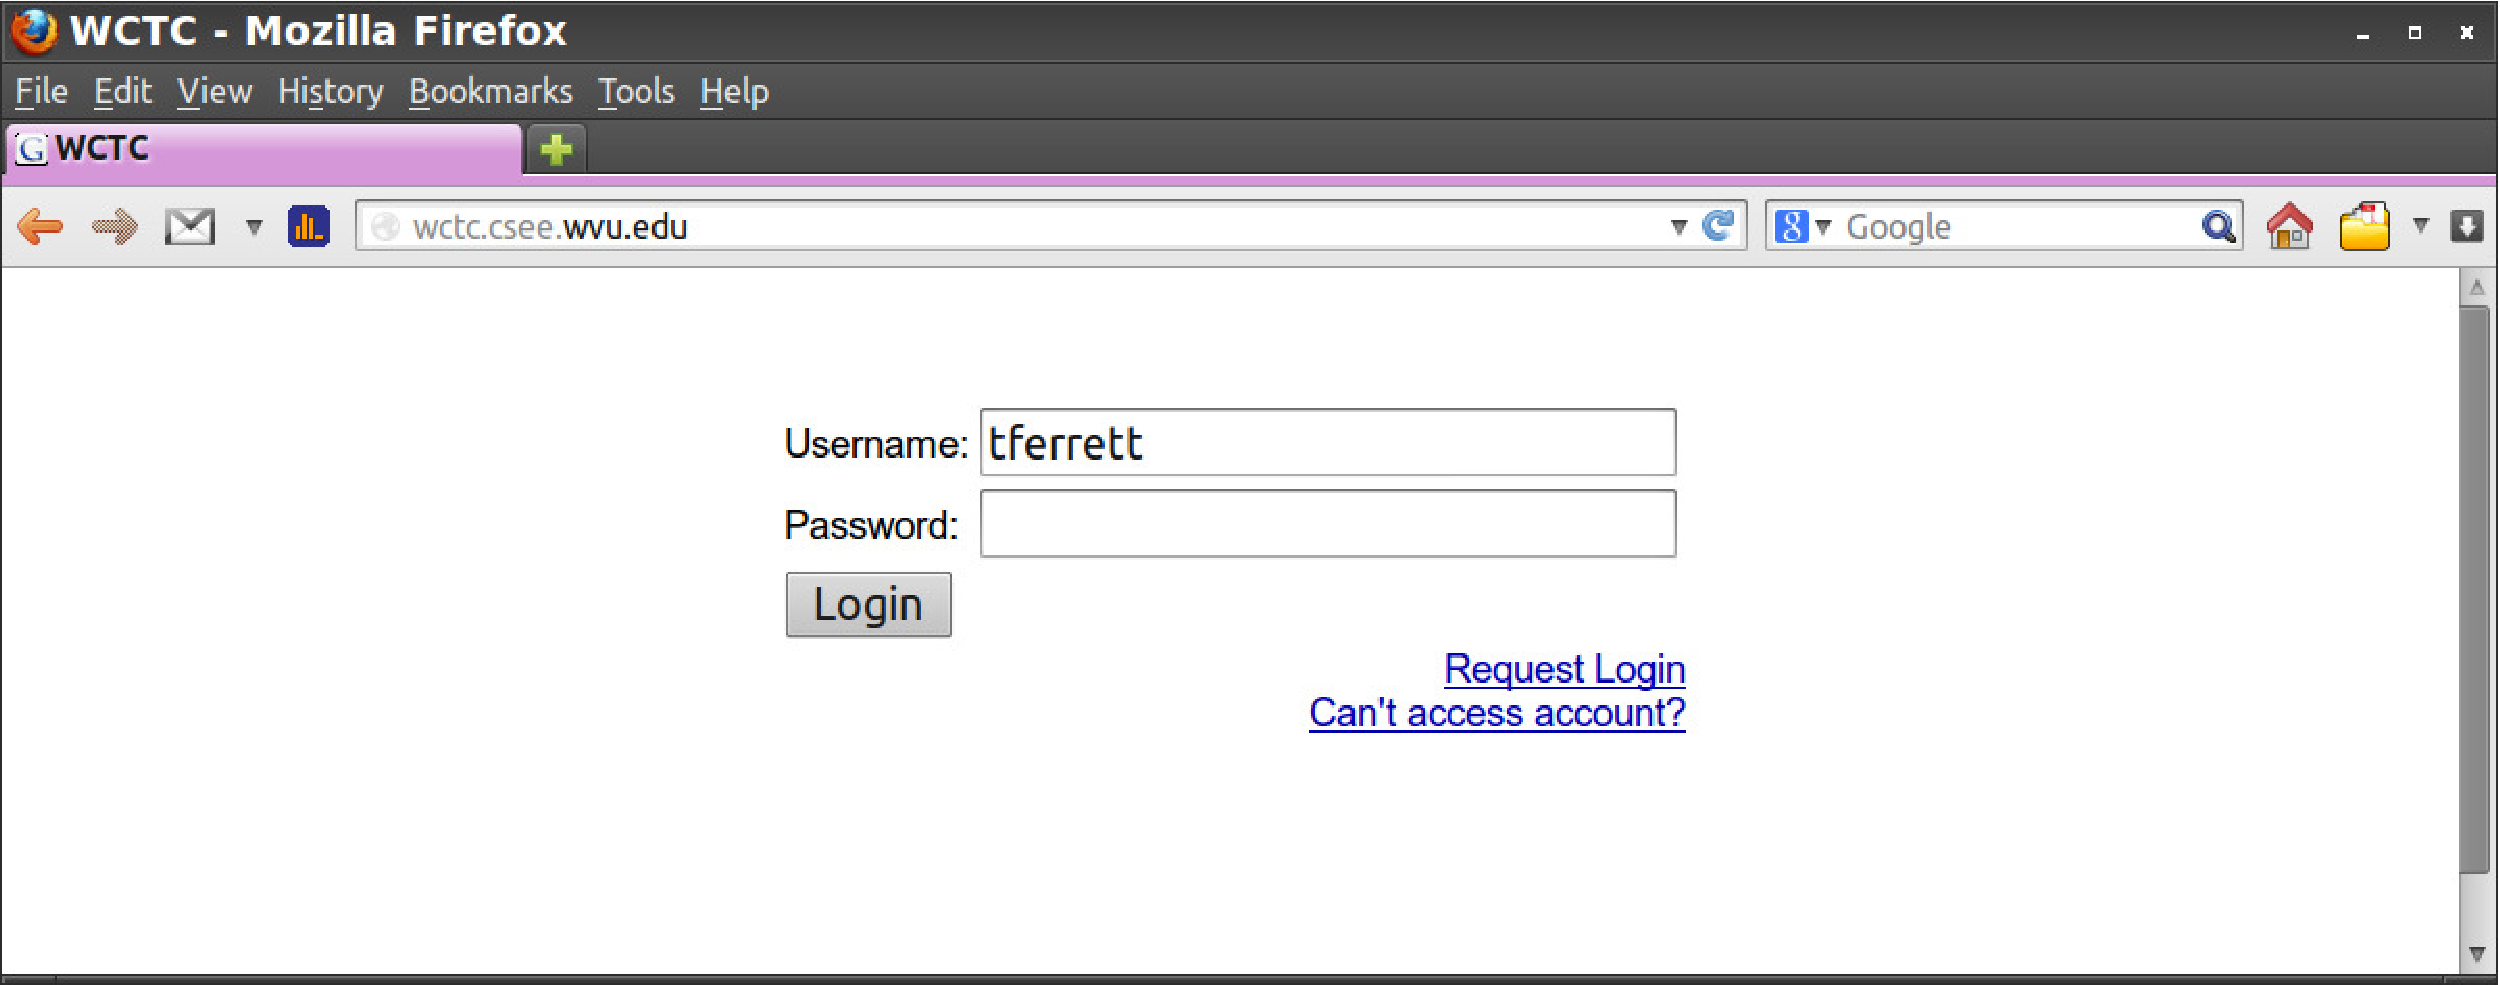
\includegraphics[width=0.9\textwidth]{wcrlctc_login}
  \end{figure}

\end{frame}




% job file submission
\begin{frame}
  \frametitle{Job File Submission}

  In this step we will add the job file to the input queue for execution.
  \begin{itemize}
  \item Click the tab ``My Jobs'', bringing up the job manipulation interface.
  \item In the drop-down next to the button ``Add Job'', select project ``cml''.
  \item Click the button ``Add Job'' as shown in the figure.
  \end{itemize}

  \centering

  \begin{figure}
    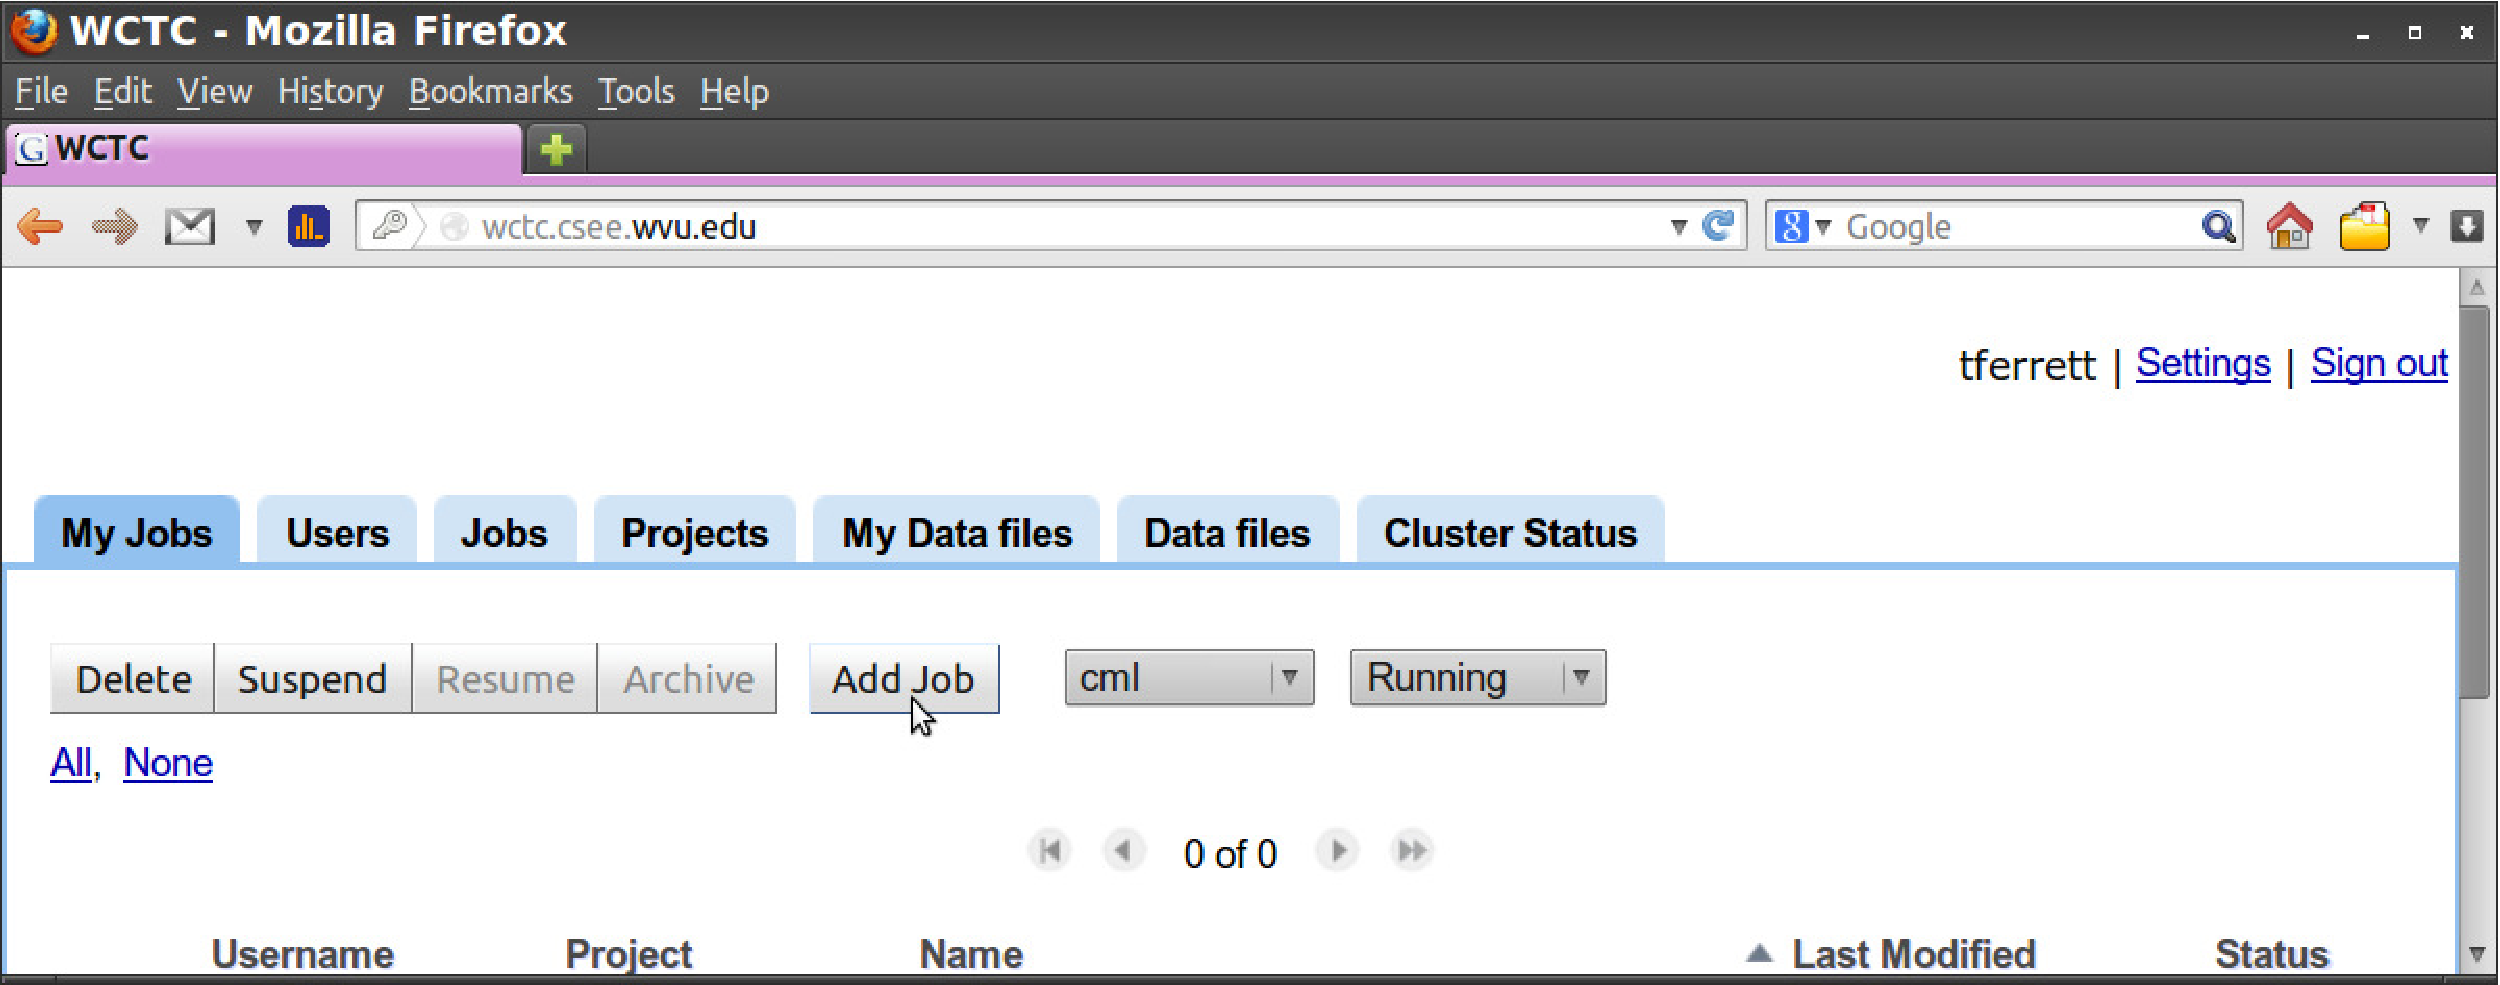
\includegraphics[width=0.9\textwidth]{wcrlctc_addjob}
  \end{figure}

\end{frame}




% file submission interface
\begin{frame}

  Select the job file to upload from the local filesystem.
  \begin{itemize}
  \item Click the ``Browse'' button. This will open a file selection dialog.
  \item Select the job file $<$CMLROOT$>$/jobs/JobIn/UncodedScenarios\_1.mat
  \end{itemize}

  \centering
  \begin{figure}
    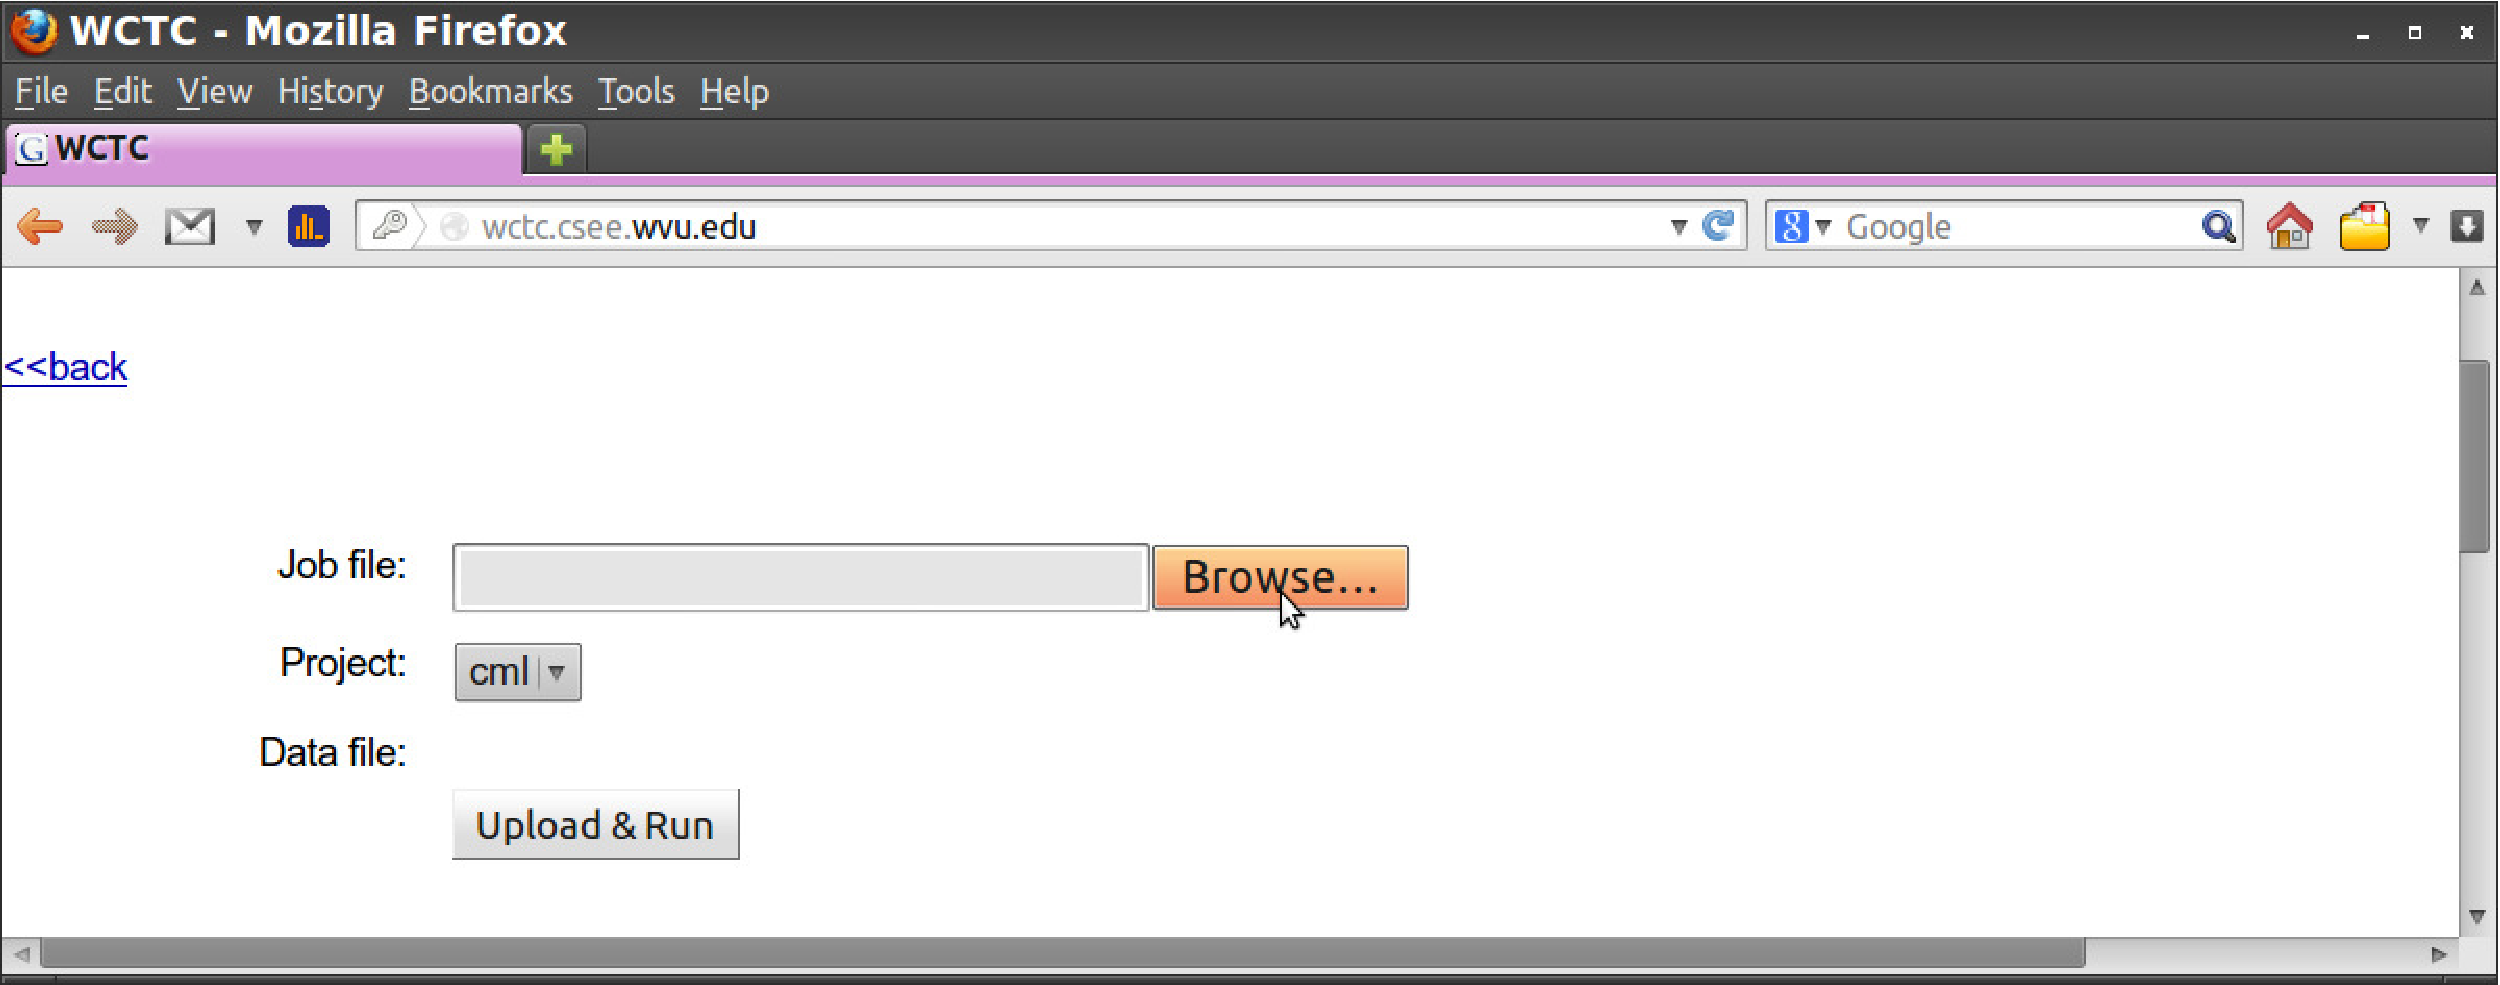
\includegraphics[width=0.7\textwidth]{wcrlctc_browsejob}
  \end{figure}

  \vspace{-8mm}

  \begin{figure}
    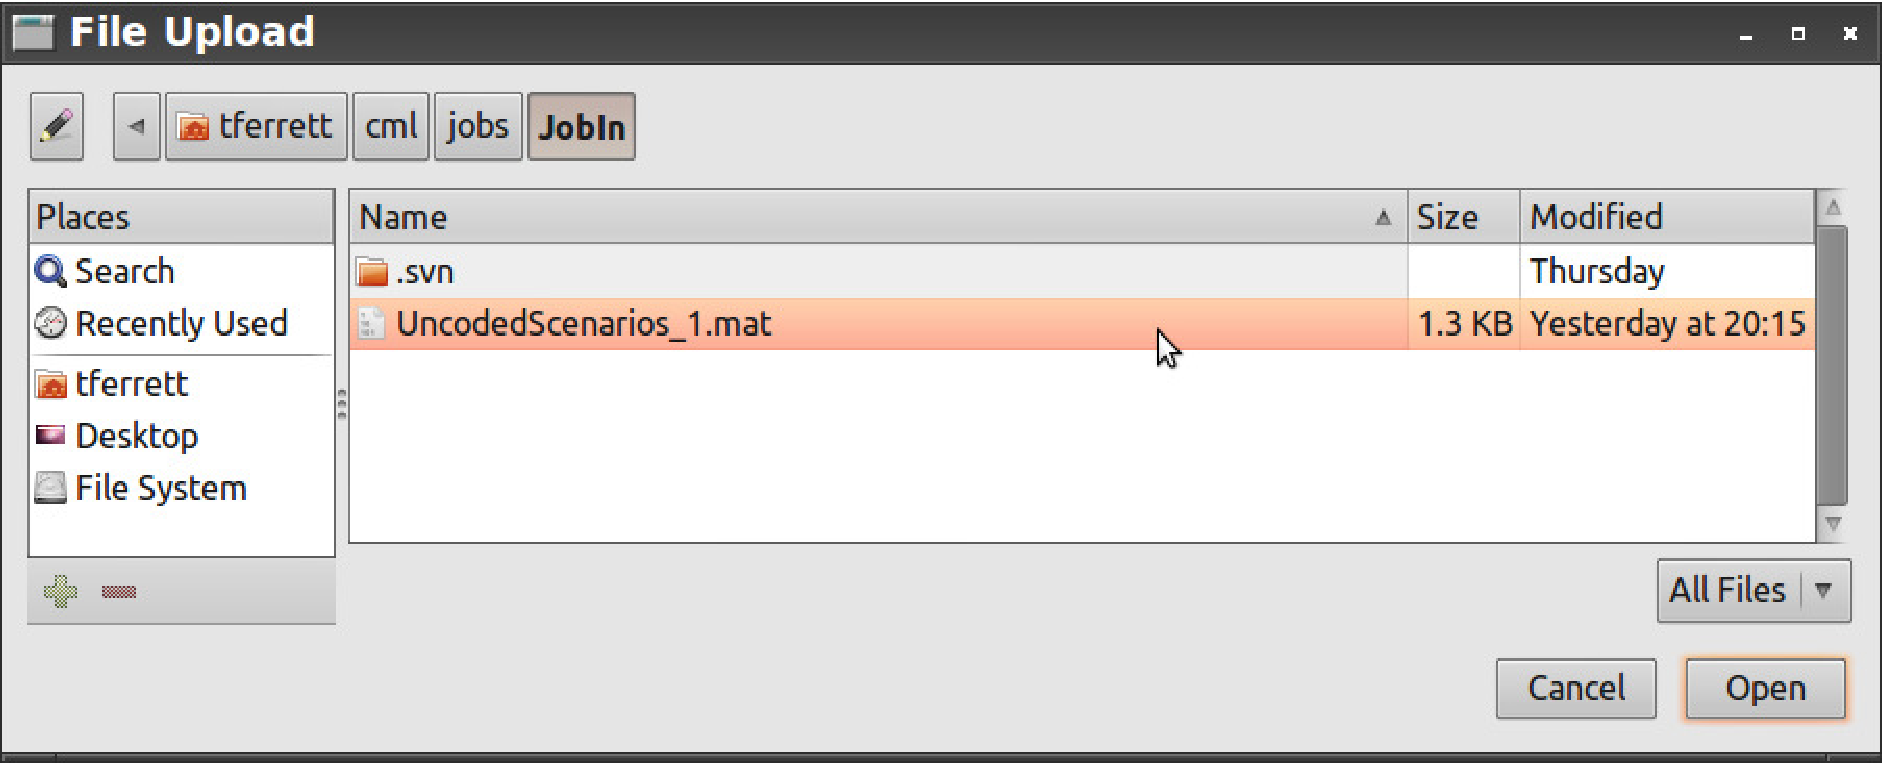
\includegraphics[width=0.7\textwidth]{wcrlctc_jobfile}
  \end{figure}

\end{frame}




% upload and run
\begin{frame}

  Uploading and running the job file submits the job to the cluster input queue for execution.
  \begin{itemize}
  \item Click ``Upload $\&$ Run'' to submit the job to the input queue.
  \end{itemize}

  \centering
  \begin{figure}
    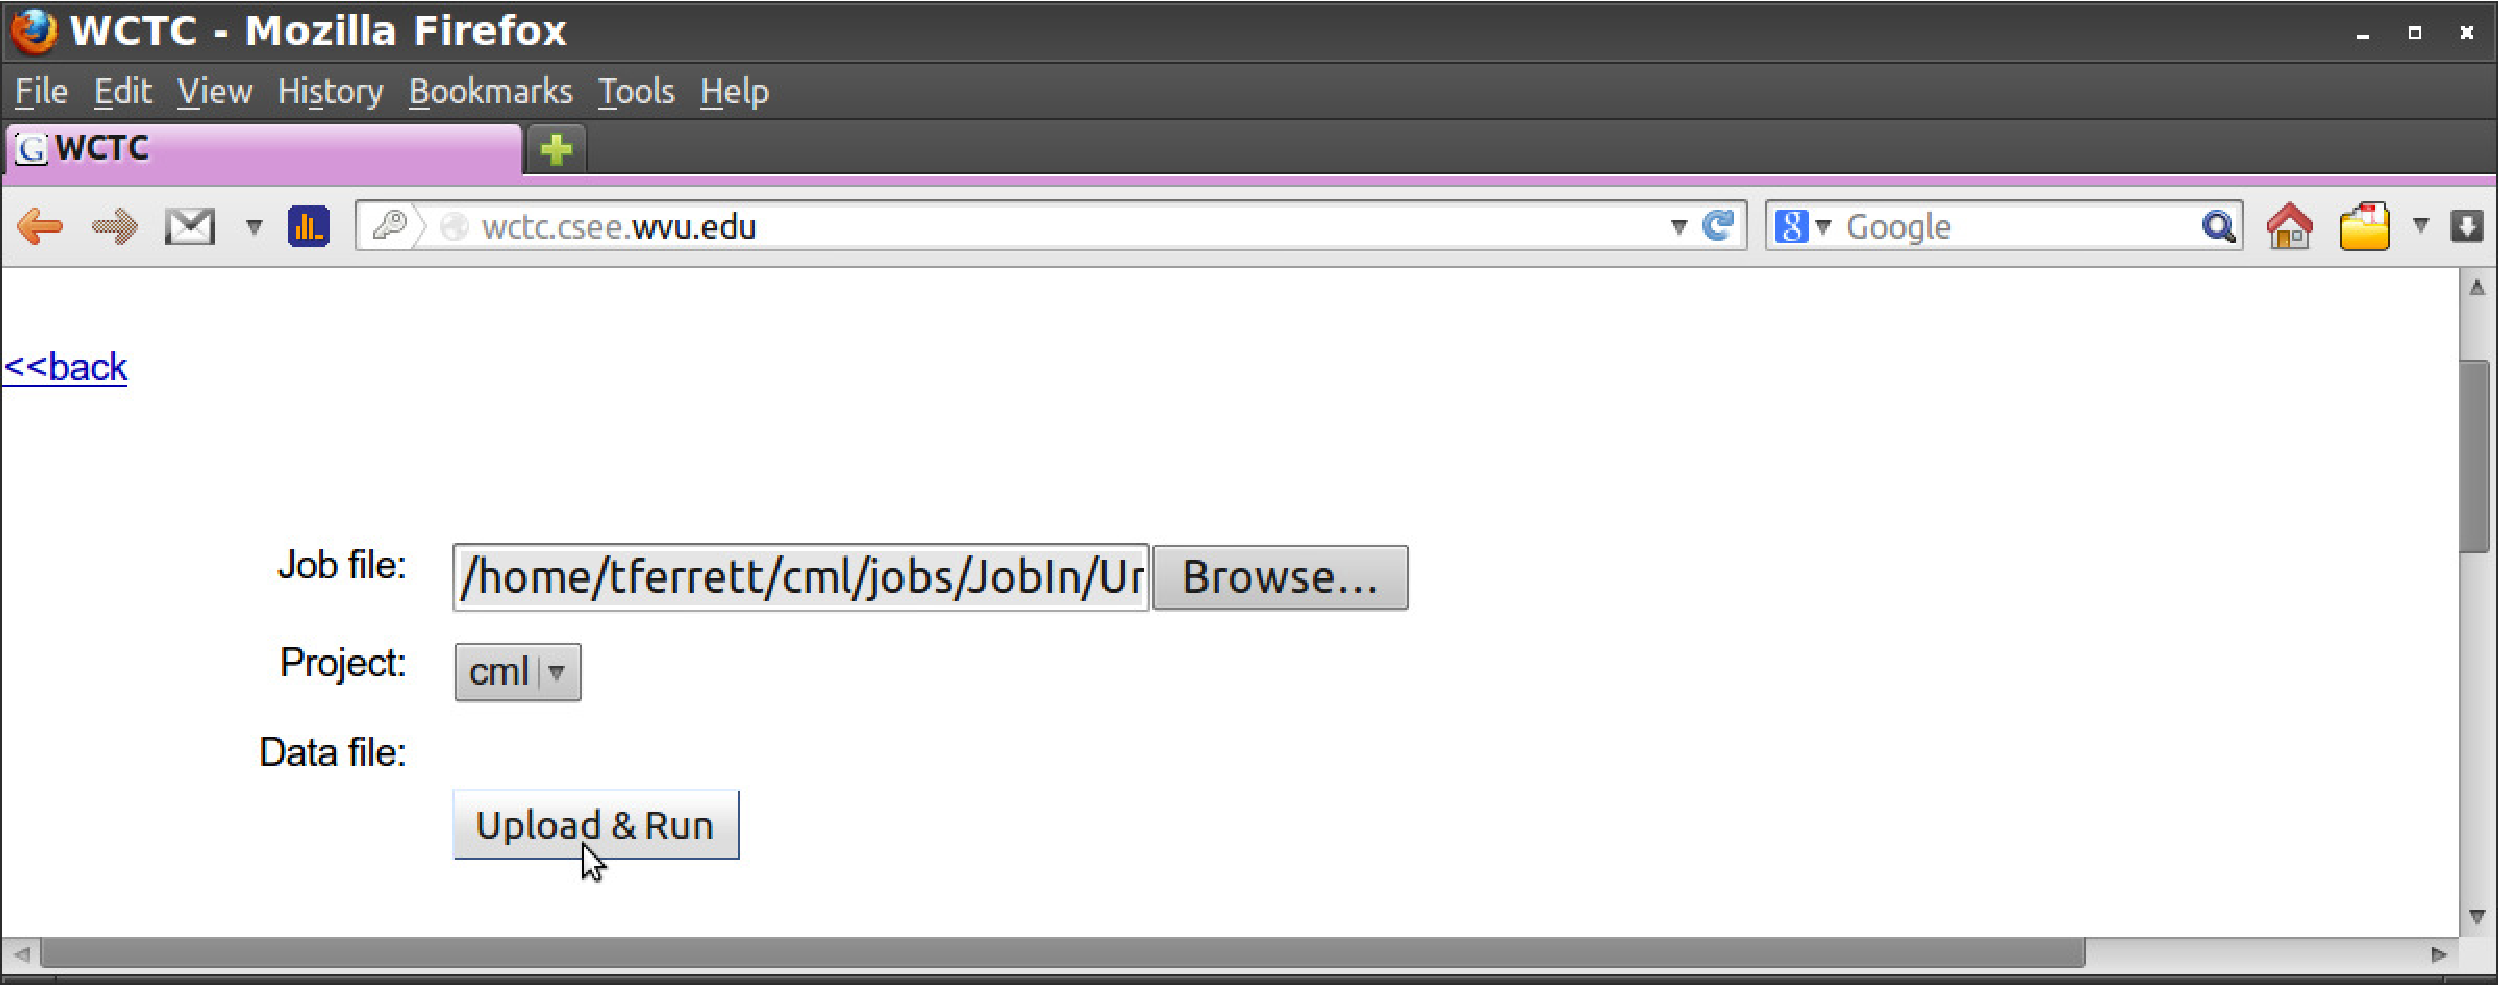
\includegraphics[width=0.9\textwidth]{wcrlctc_upload}
  \end{figure}

\end{frame}




% job execution
\begin{frame}
  \frametitle{Job Execution}

  The job is now executed on the cluster when resources are available.\\
  To check for job completion,

  \begin{itemize}
  \item In the drop-down menu highlighted in the figure, select ``Done''.  
  \item The completed job will appear in the table at the bottom of the page, as shown in the figure.
  \end{itemize}

  \begin{figure}
    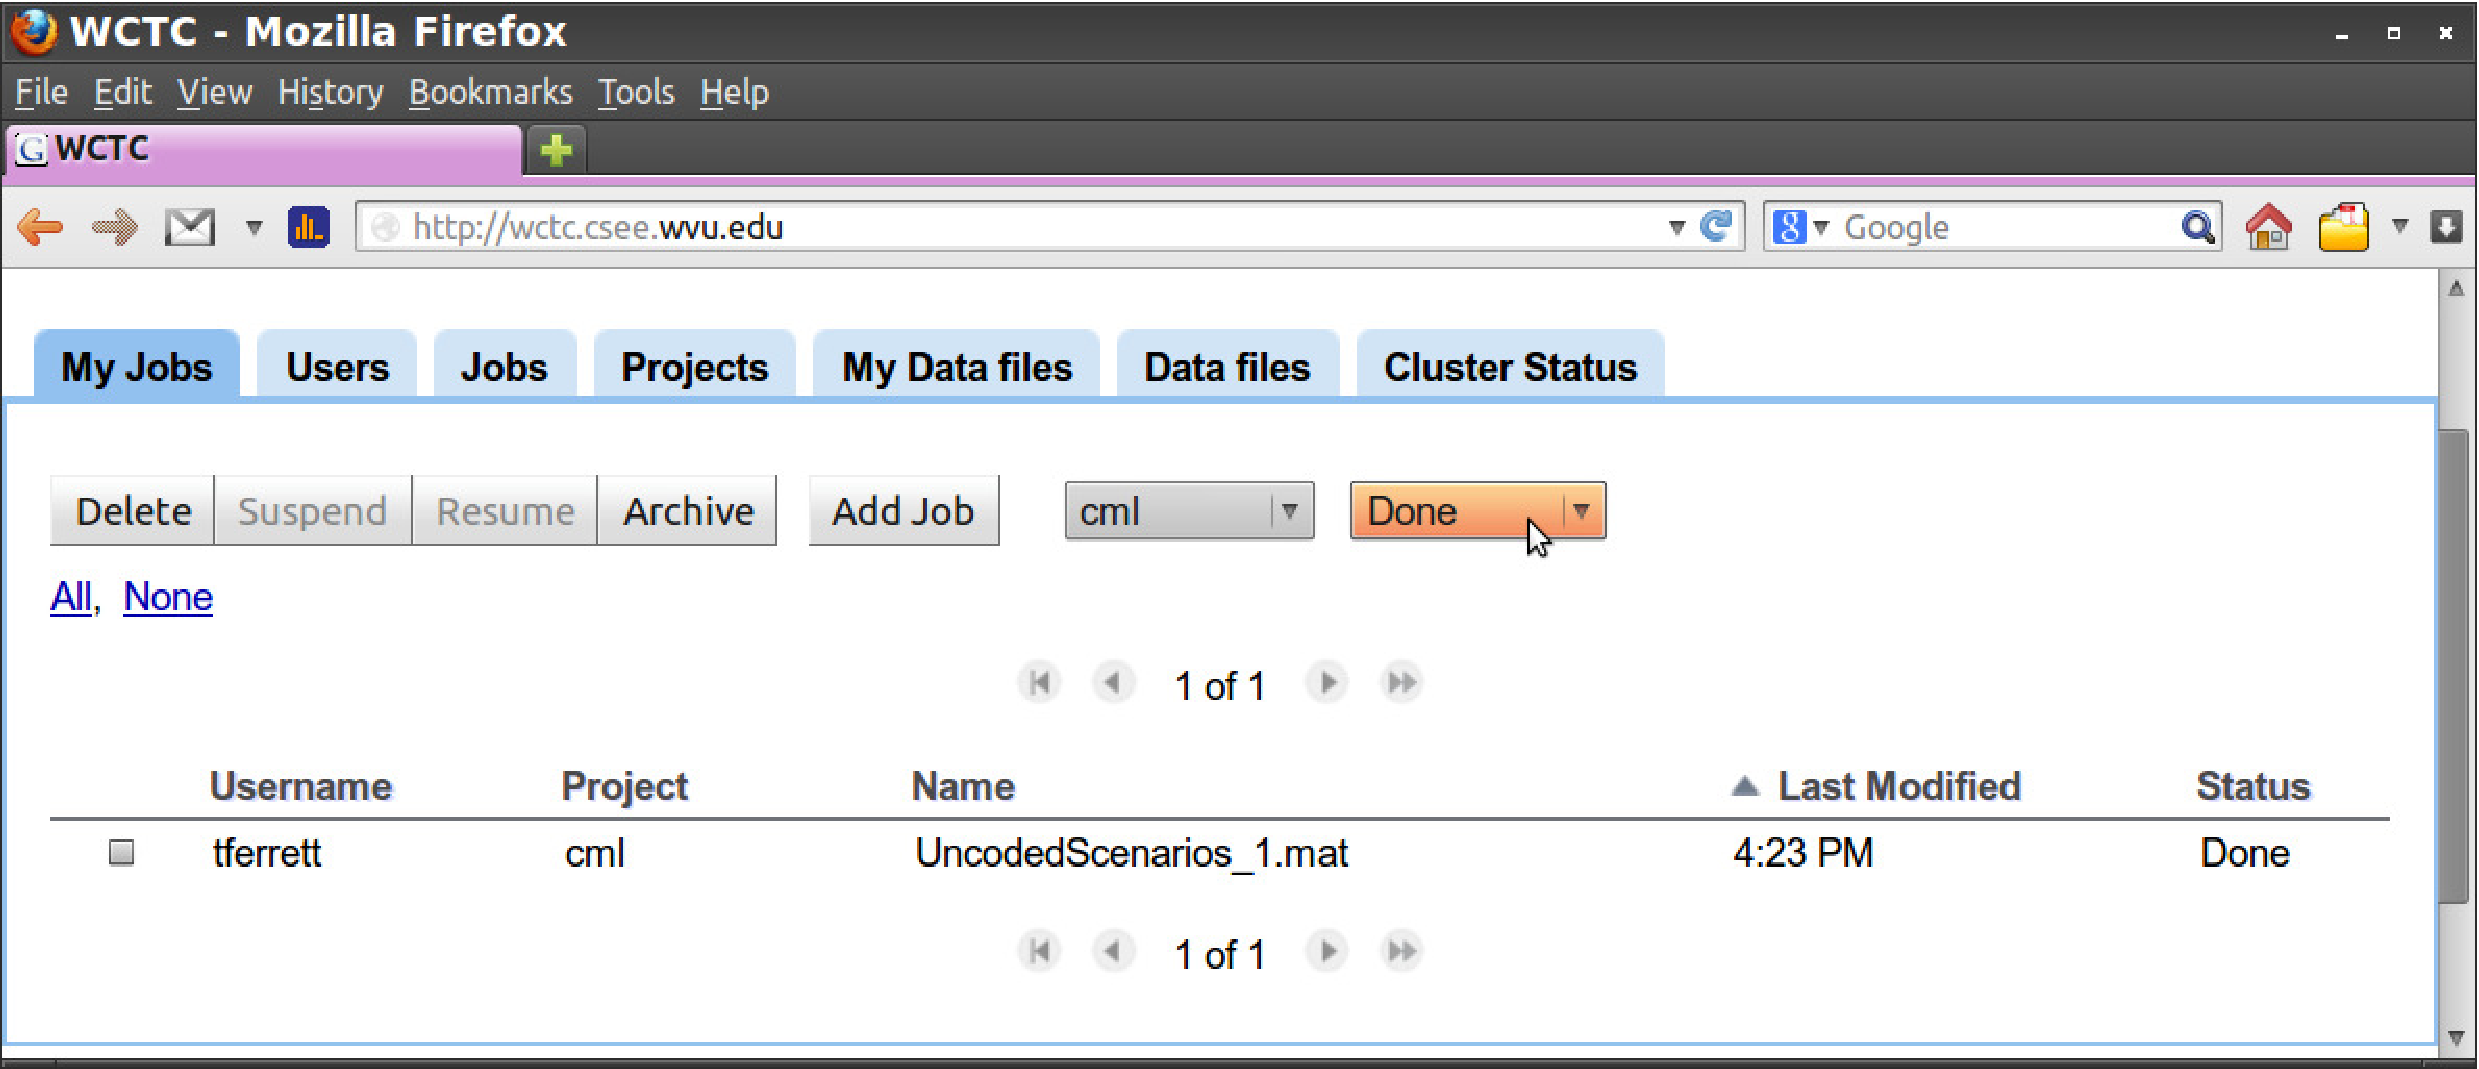
\includegraphics[width=0.9\textwidth]{wcrlctc_done}
  \end{figure}

\end{frame}




% results retrieval
\begin{frame}
  \frametitle{Job Results Retrieval}

  Now that the job is complete, retrieve the results for local plotting.
  \begin{itemize}
  \item Click the link to the name of the job file as shown in the figure and perform a ``Save As'' operation.
  \end{itemize}

  \centering
  \begin{figure}
    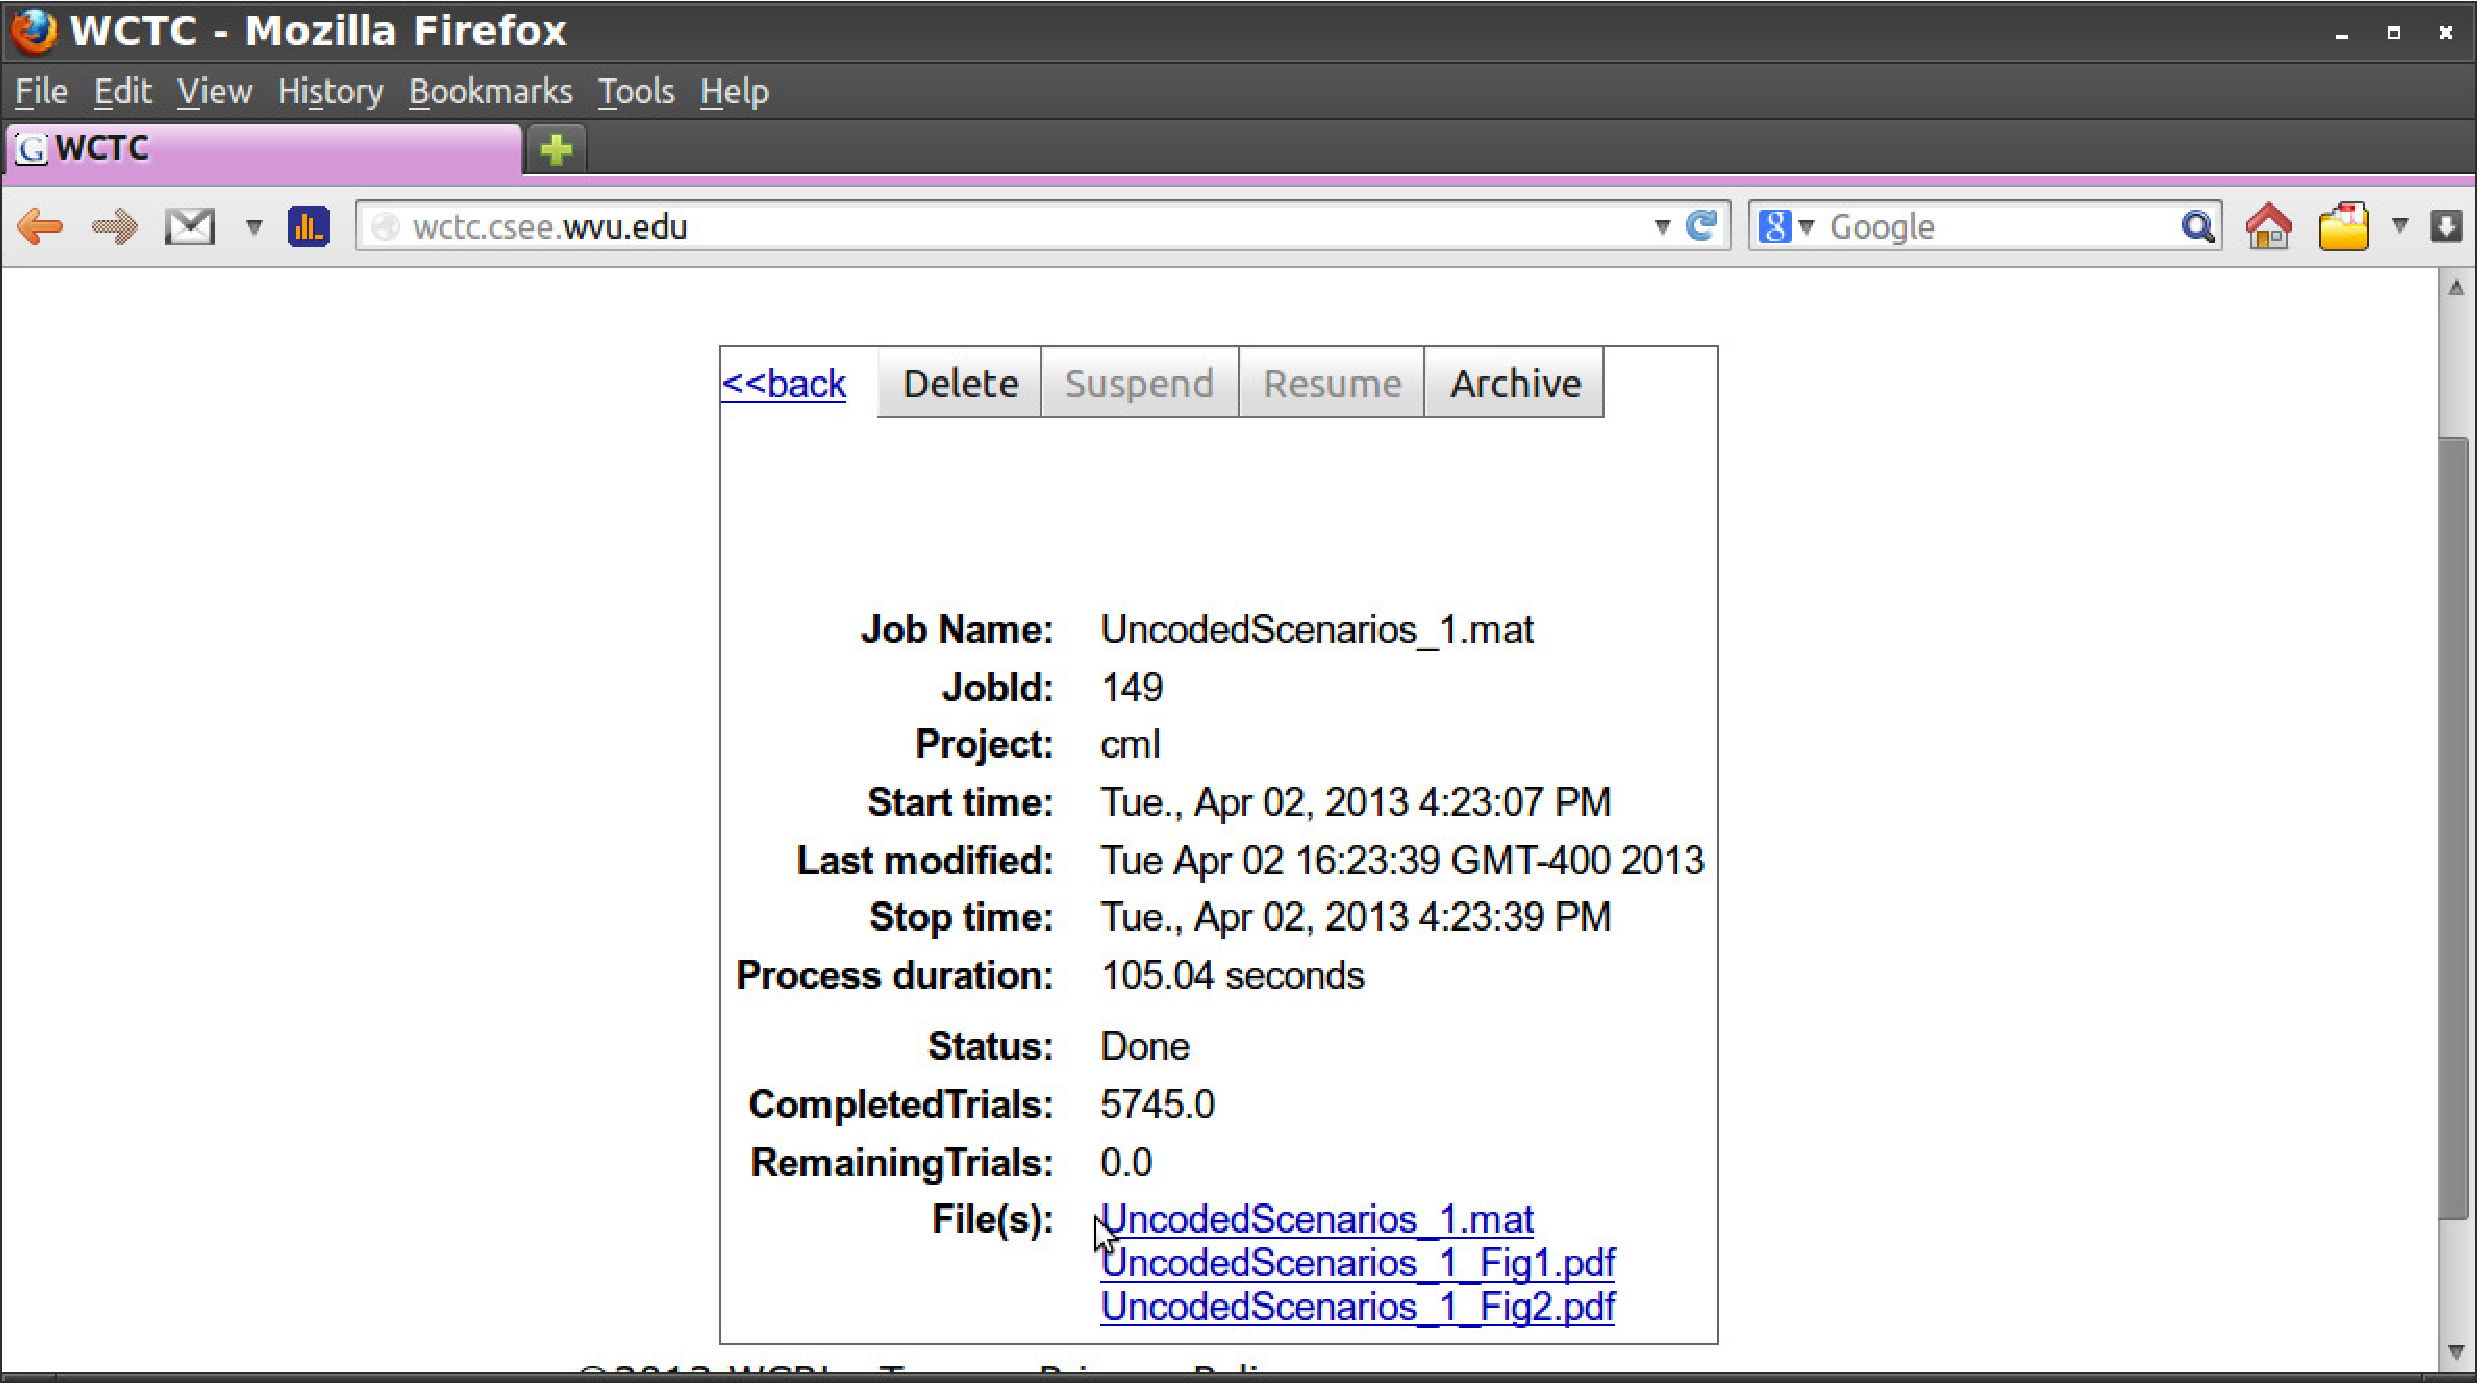
\includegraphics[width=0.9\textwidth]{wcrlctc_downjob}
  \end{figure}

\end{frame}




% saving to jobout
\begin{frame}

  \begin{itemize_loose}
  \item All completed jobs must be placed in $<$CMLROOT$>$/jobs/JobOut for processing
    by CML.
  \item When prompted for a location to save the completed job file, specify
    \begin{itemize}
    \item $<$CMLROOT$>$/jobs/JobOut/UncodedScenarios\_1.mat
    \end{itemize}
    as shown in the figure.
  \end{itemize_loose}

  \centering
  \begin{figure}
    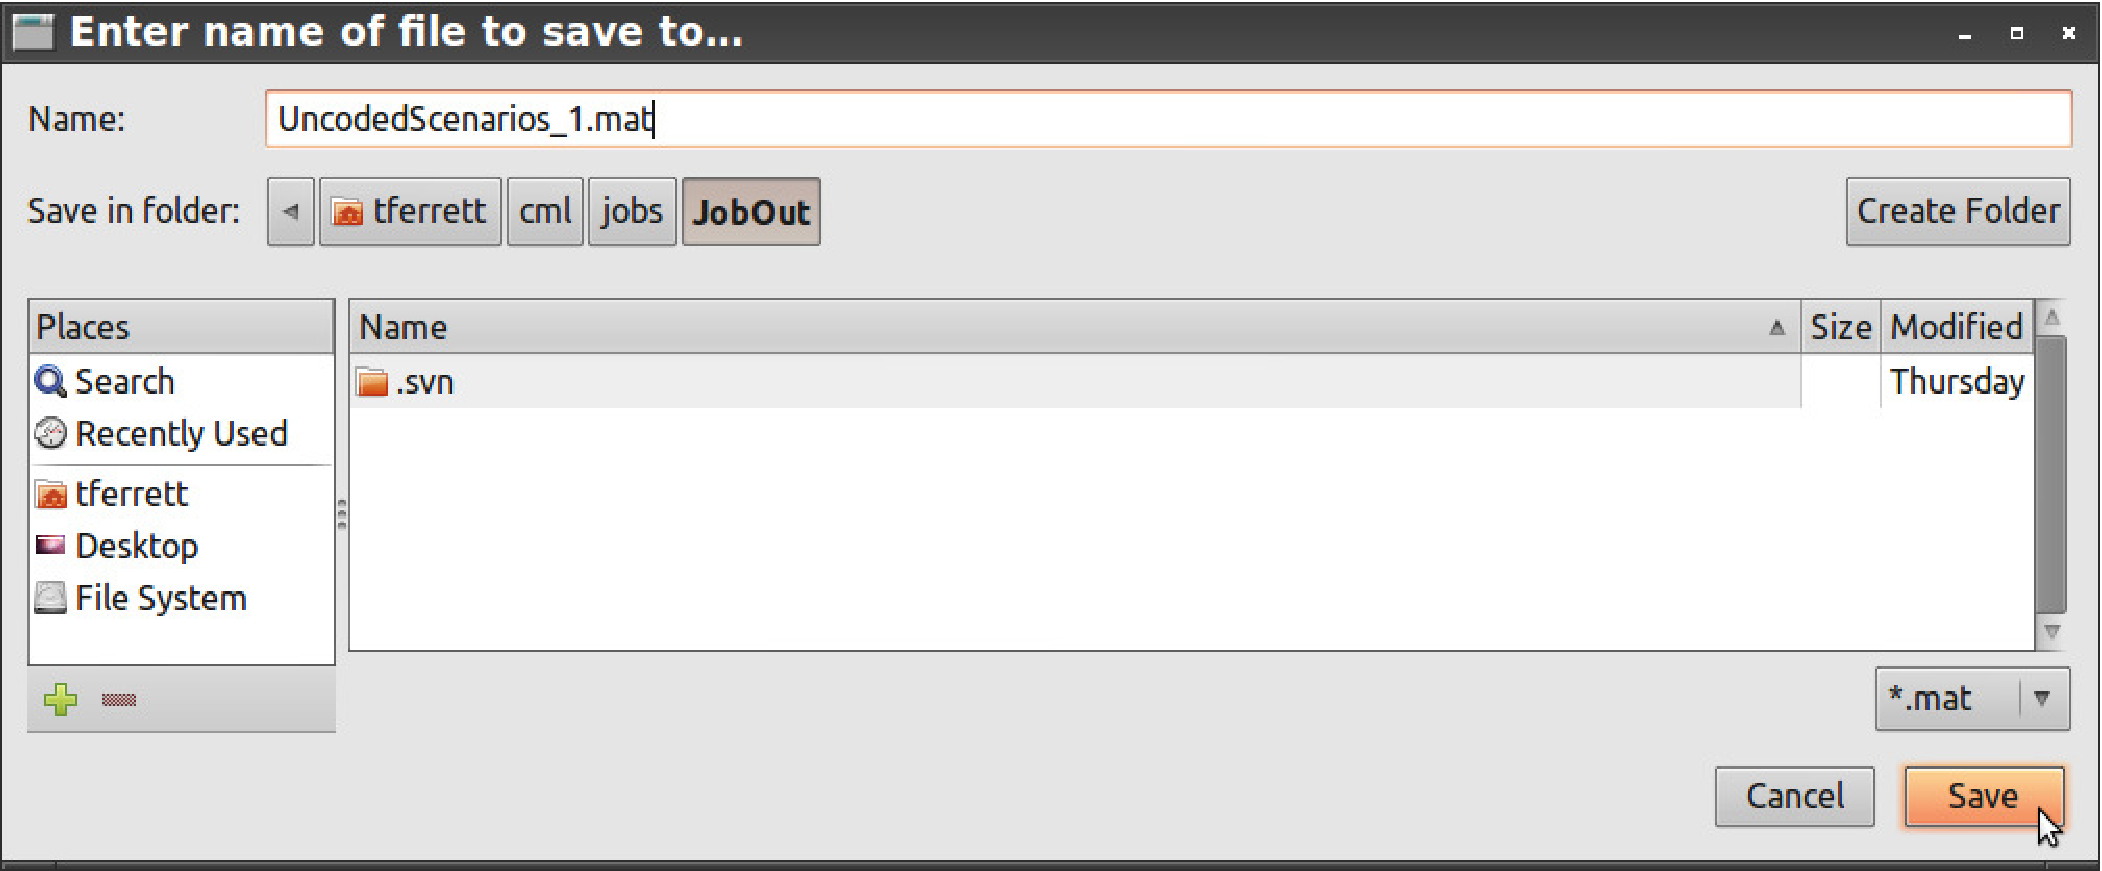
\includegraphics[width=0.9\textwidth]{wcrlctc_jobout}
  \end{figure}

\end{frame}




% cmlwebretrieve
\begin{frame}
  \frametitle{Job File Conversion and Result Plotting}

  The completed job file must be converted to a CML output file appropriate for plotting.
  \begin{itemize}
  \item Execute the function 'CmlWebRetrieve' to convert the job file to a CML output file as shown in the figure.
  \item The results of simulation may now be plotted as shown.
  \end{itemize}

  \centering
  \begin{figure}
    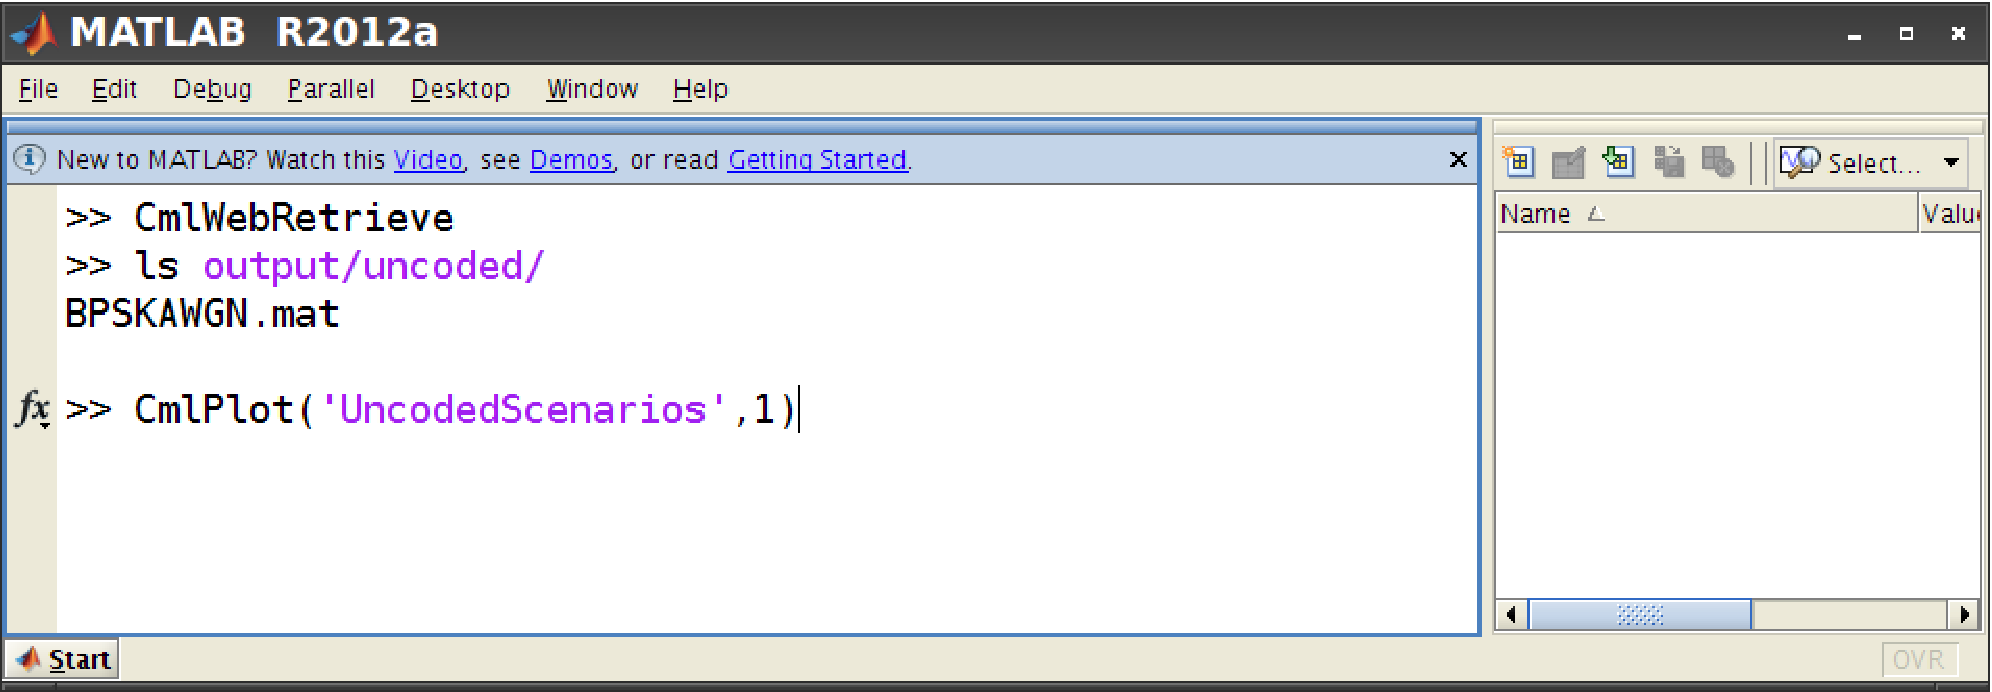
\includegraphics[width=0.9\textwidth]{cml_webretrieve}
  \end{figure}

\end{frame}



% plotted results
\begin{frame}

  \centering
  \begin{figure}
    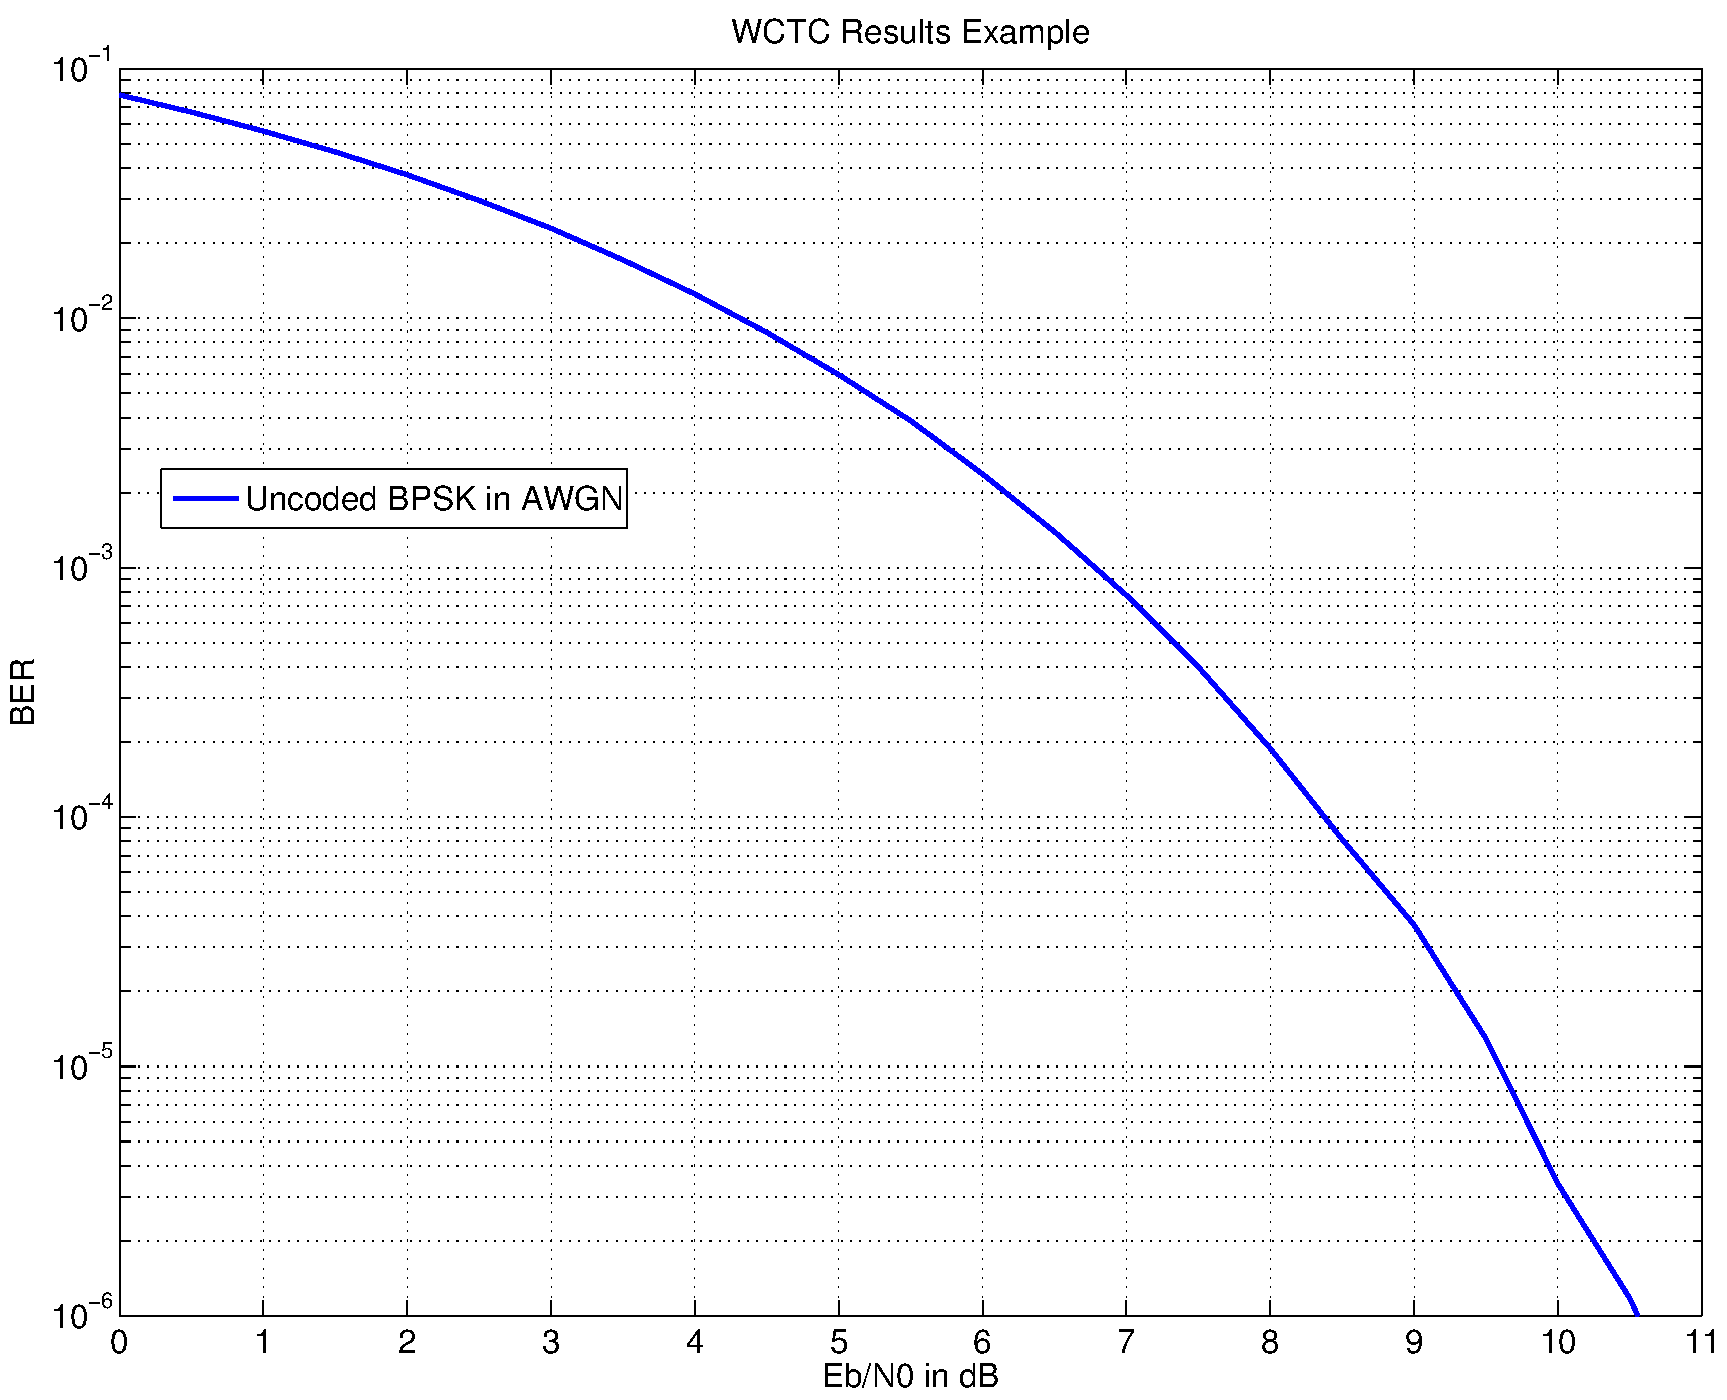
\includegraphics[width=0.8\textwidth]{cml_res}
  \end{figure}

\end{frame}





